% !TeX root = ../main.tex
\section{Experiments}
\label{sec:experiments}
\setcounter{dbltopnumber}{2}

\subsection{Experimental setup}
\label{sec:experiment_setup}

We initialize our model from Wan2.2-TI2V-5B and train with BF16 precision, keeping the VAE and text encoder frozen.
Training clips contain 81 frames at 16\,fps, with RGB resolution $832\!\times\!480$ and depth resolution $448\!\times\!256$.
We train the bidirectional model for 2 epochs with a batch size of 64, followed by 250 steps of causal post-training with a batch size of 256.

We select subsets from multiple data sources, yielding 1,350 evaluation clips in total.
Each clip contains 81 frames at 16\,fps.

We compare with text-and-image-to-video (TI2V) world models: SolarWM-5B SGF Stage~2~\cite{huang2026solarwmopendatascalable} and the Hunyuan DMD variant of minWM~\cite{zhao2026minwmfullstackopensourceframework}.
All compared models generate videos conditioned on an initial RGB frame, a text prompt, and a camera trajectory through their native conditioning interfaces.
For the quantitative comparison, our model and SolarWM use four denoising steps at $832\!\times\!480$ and $864\!\times\!480$, respectively; pixel-level references follow the corresponding native preprocessing.
For minWM, we retain its native camera-translation normalization.
% Evaluated weights: our DF step252 raw checkpoint; official SolarWM Stage2 EMA.
% minWM results come from the author-supplied three-model-metrics.json.
% The matching minWM full-scaled outputs and ViPE summary were verified on
% AutoDL; per-clip translation normalization is retained in those outputs.

For visual fidelity, we report LPIPS with AlexNet features~\cite{zhang2018lpips} and FVD~\cite{unterthiner2018fvd}.
LPIPS excludes the conditioning frame, with equal weighting across clips.
FVD uses all 81 frames and a shared 400-dimensional pre-softmax I3D representation at $224\!\times\!224$ resolution.

For camera control, ViPE~\cite{huang2025vipevideoposeengine} recovers trajectories from generated RGB, independently of our predicted depth.
We report SCoPE's framewise RotErr (degrees), TransErr, and CamMC~\cite{yin2026scope}, supplemented by pose-matrix cosine similarity (CosSim) and all-pairs relative-pose AUC at $15^\circ$/$30^\circ$~\cite{wang2025vggt}.
Trajectories are anchored at the first frame and translations independently normalized by maximum displacement; these scores assess relative motion rather than absolute scale.

\subsection{Annotation pipeline evaluation}
\label{sec:annotation_evaluation}

Conventional SfM and learning-based estimators offer several routes to camera annotation, but reference trajectories are generally unavailable for web videos.
Our camera-pipeline validation uses 16 clips, comprising 12 GTA clips and four real-world clips.
The simulator provides diverse scenes, realistic imagery, and recorded trajectories, enabling comparisons of reconstruction quality, runtime, and scale recovery.
We first compare reconstruction strategies and then examine scale accuracy to select the hybrid pipeline in Sec.~\ref{sec:camera_annotation}.

\paragraph{Reconstruction and scale.}
Table~\ref{tab:pose_coverage} compares SIFT and LightGlue with COLMAP against Pi3X initialized reconstruction with shared-intrinsics BA.
Pi3X produces complete outputs for all 16 clips in a median of 26.69 seconds, compared with 140.86 seconds for SIFT and 94.71 seconds for LightGlue.
SIFT has the lowest median ATE on the common valid subset, while Pi3X has the lowest P90 error.
The higher cost of conventional SfM therefore yields inconsistent accuracy gains, motivating learned initialization for large-scale annotation.

\begin{table}[htbp]
    \centering
    \caption{SfM versus learned reconstruction. Complete outputs and median runtime use all 16 clips. Sim3 ATE is camera-center RMSE in reference-trajectory units on seven common valid clips.}
    \label{tab:pose_coverage}
    \small
    \setlength{\tabcolsep}{3pt}
    \begin{tabular}{lrrr}
        \toprule
        Method & Full & Time (s) $\downarrow$ & \shortstack{ATE $\downarrow$\\median / P90} \\
        \midrule
        SIFT + COLMAP & 10/16 & 140.86 & \textbf{0.04125} / 1.40108 \\
        LightGlue + COLMAP & 13/16 & 94.71 & 0.88925 / 4.47273 \\
        Pi3X + BA & \textbf{16/16} & \textbf{26.69} & 0.06356 / \textbf{0.10589} \\
        \bottomrule
    \end{tabular}
\end{table}

Among learned methods, Pi3X and ViPE~\cite{huang2025vipevideoposeengine} both recover accurate relative geometry after scale alignment (Table~\ref{tab:learned_geometry}).
Their median normalized ATE is 0.083--0.127\% and rotation error is approximately $0.46^\circ$, while scale errors remain 20.64--22.17\% under a common UniDepthV2 backend.
We retain Pi3X for its complete-frame coverage and focus further comparison on translation scale, which determines the magnitude of camera-motion supervision.
Native Pi3X alone has a 38.87\% median scale error on an eight-clip ablation subset, motivating the additional geometric refinement and calibrated scale recovery detailed in the Supplementary Material.

\begin{table}[htbp]
    \centering
    \caption{Relative geometry and scale. Error medians use 14 common successful clips. Sim3 ATE is normalized by reference path length, while coverage uses all 16 clips.}
    \label{tab:learned_geometry}
    \small
    \setlength{\tabcolsep}{3pt}
    \begin{tabular}{lrrrr}
        \toprule
        Geometry & Full & ATE (\%) $\downarrow$ & Rot. ($^\circ$) $\downarrow$ & Scale (\%) $\downarrow$ \\
        \midrule
        Pi3X + BA & \textbf{16/16} & 0.127 & 0.460 & 22.17 \\
        ViPE + BA & 14/16 & 0.125 & 0.459 & \textbf{20.64} \\
        ViPE, native & 14/16 & \textbf{0.083} & \textbf{0.455} & 21.30 \\
        \bottomrule
    \end{tabular}
\end{table}

\begin{table}[htbp]
    \centering
    \caption{Calibrated scale recovery with fixed geometry. Median and P90 scale errors use 15 scorable outputs from 16 attempted clips with frozen parameters.}
    \label{tab:scale_selection}
    \small
    \setlength{\tabcolsep}{3pt}
    \begin{tabular}{lrr}
        \toprule
        Scale configuration & Median (\%) $\downarrow$ & P90 (\%) $\downarrow$ \\
        \midrule
        UniDepthV2, P98 baseline & 25.46 & 51.65 \\
        + inverse-depth correction & \textbf{22.40} & \textbf{45.60} \\
        \bottomrule
    \end{tabular}
\end{table}

Holding geometry and intrinsics fixed, inverse-depth correction reduces median scale error from 25.46\% to 22.40\% and P90 from 51.65\% to 45.60\% (Table~\ref{tab:scale_selection}).
It achieves the lowest median error among the evaluated scale configurations, whose complete comparison appears in the Supplementary Material.
The remaining scale error highlights the importance of directly recorded camera trajectories and depth for geometric supervision, together with real-flight observations of the intended operating conditions.

\begin{table}[htbp]
    \centering
    \caption{Depth annotation on 16 GTA clips. AbsRel and RMSE use the 0.1--80\,m range. Temporal log-depth error uses motion-compensated correspondences over 0.1--1,000\,m. Lower is better.}
    \label{tab:depth_annotation_selection}
    \small
    \setlength{\tabcolsep}{3pt}
    \begin{tabular}{@{}lrrr@{}}
        \toprule
        Configuration & AbsRel (\%) & RMSE (m) & Temporal \\
        \midrule
        MetricAnything & \textbf{17.69} & \textbf{9.54} & 0.03759 \\
        + VDA stabilization & 18.20 & 9.63 & \textbf{0.02124} \\
        \bottomrule
    \end{tabular}
\end{table}

\begin{table*}[t]
    \centering
    \caption{Quantitative comparison with TI2V world models on 1,350 clips. We evaluate visual fidelity and camera-trajectory adherence, with camera control measured from ViPE-recovered RGB trajectories after per-clip translation normalization. Best results are bold.}
    \label{tab:main_comparison}
    \small
    \setlength{\tabcolsep}{6pt}
    \begin{tabular}{@{}lrrrrrrrr@{}}
        \toprule
        & \multicolumn{2}{c}{Visual fidelity} & \multicolumn{6}{c}{Camera control} \\
        \cmidrule(lr){2-3}\cmidrule(l){4-9}
        Method & LPIPS$\downarrow$ & FVD$\downarrow$ & RotErr$\downarrow$ & TransErr$\downarrow$ & CamMC$\downarrow$ & CosSim$\uparrow$ & AUC@15$\uparrow$ & AUC@30$\uparrow$ \\
        \midrule
        minWM & 0.515 & 302.63 & 12.132 & 0.299 & 0.453 & 0.942 & 0.141 & 0.333 \\
        SolarWM & 0.490 & 171.07 & 5.239 & 0.133 & 0.202 & 0.980 & 0.544 & 0.708 \\
        Ours & \textbf{0.373} & \textbf{51.75} & \textbf{1.945} & \textbf{0.090} & \textbf{0.111} & \textbf{0.991} & \textbf{0.695} & \textbf{0.813} \\
        \bottomrule
    \end{tabular}
\end{table*}

\begin{figure*}[!t]
    \centering
    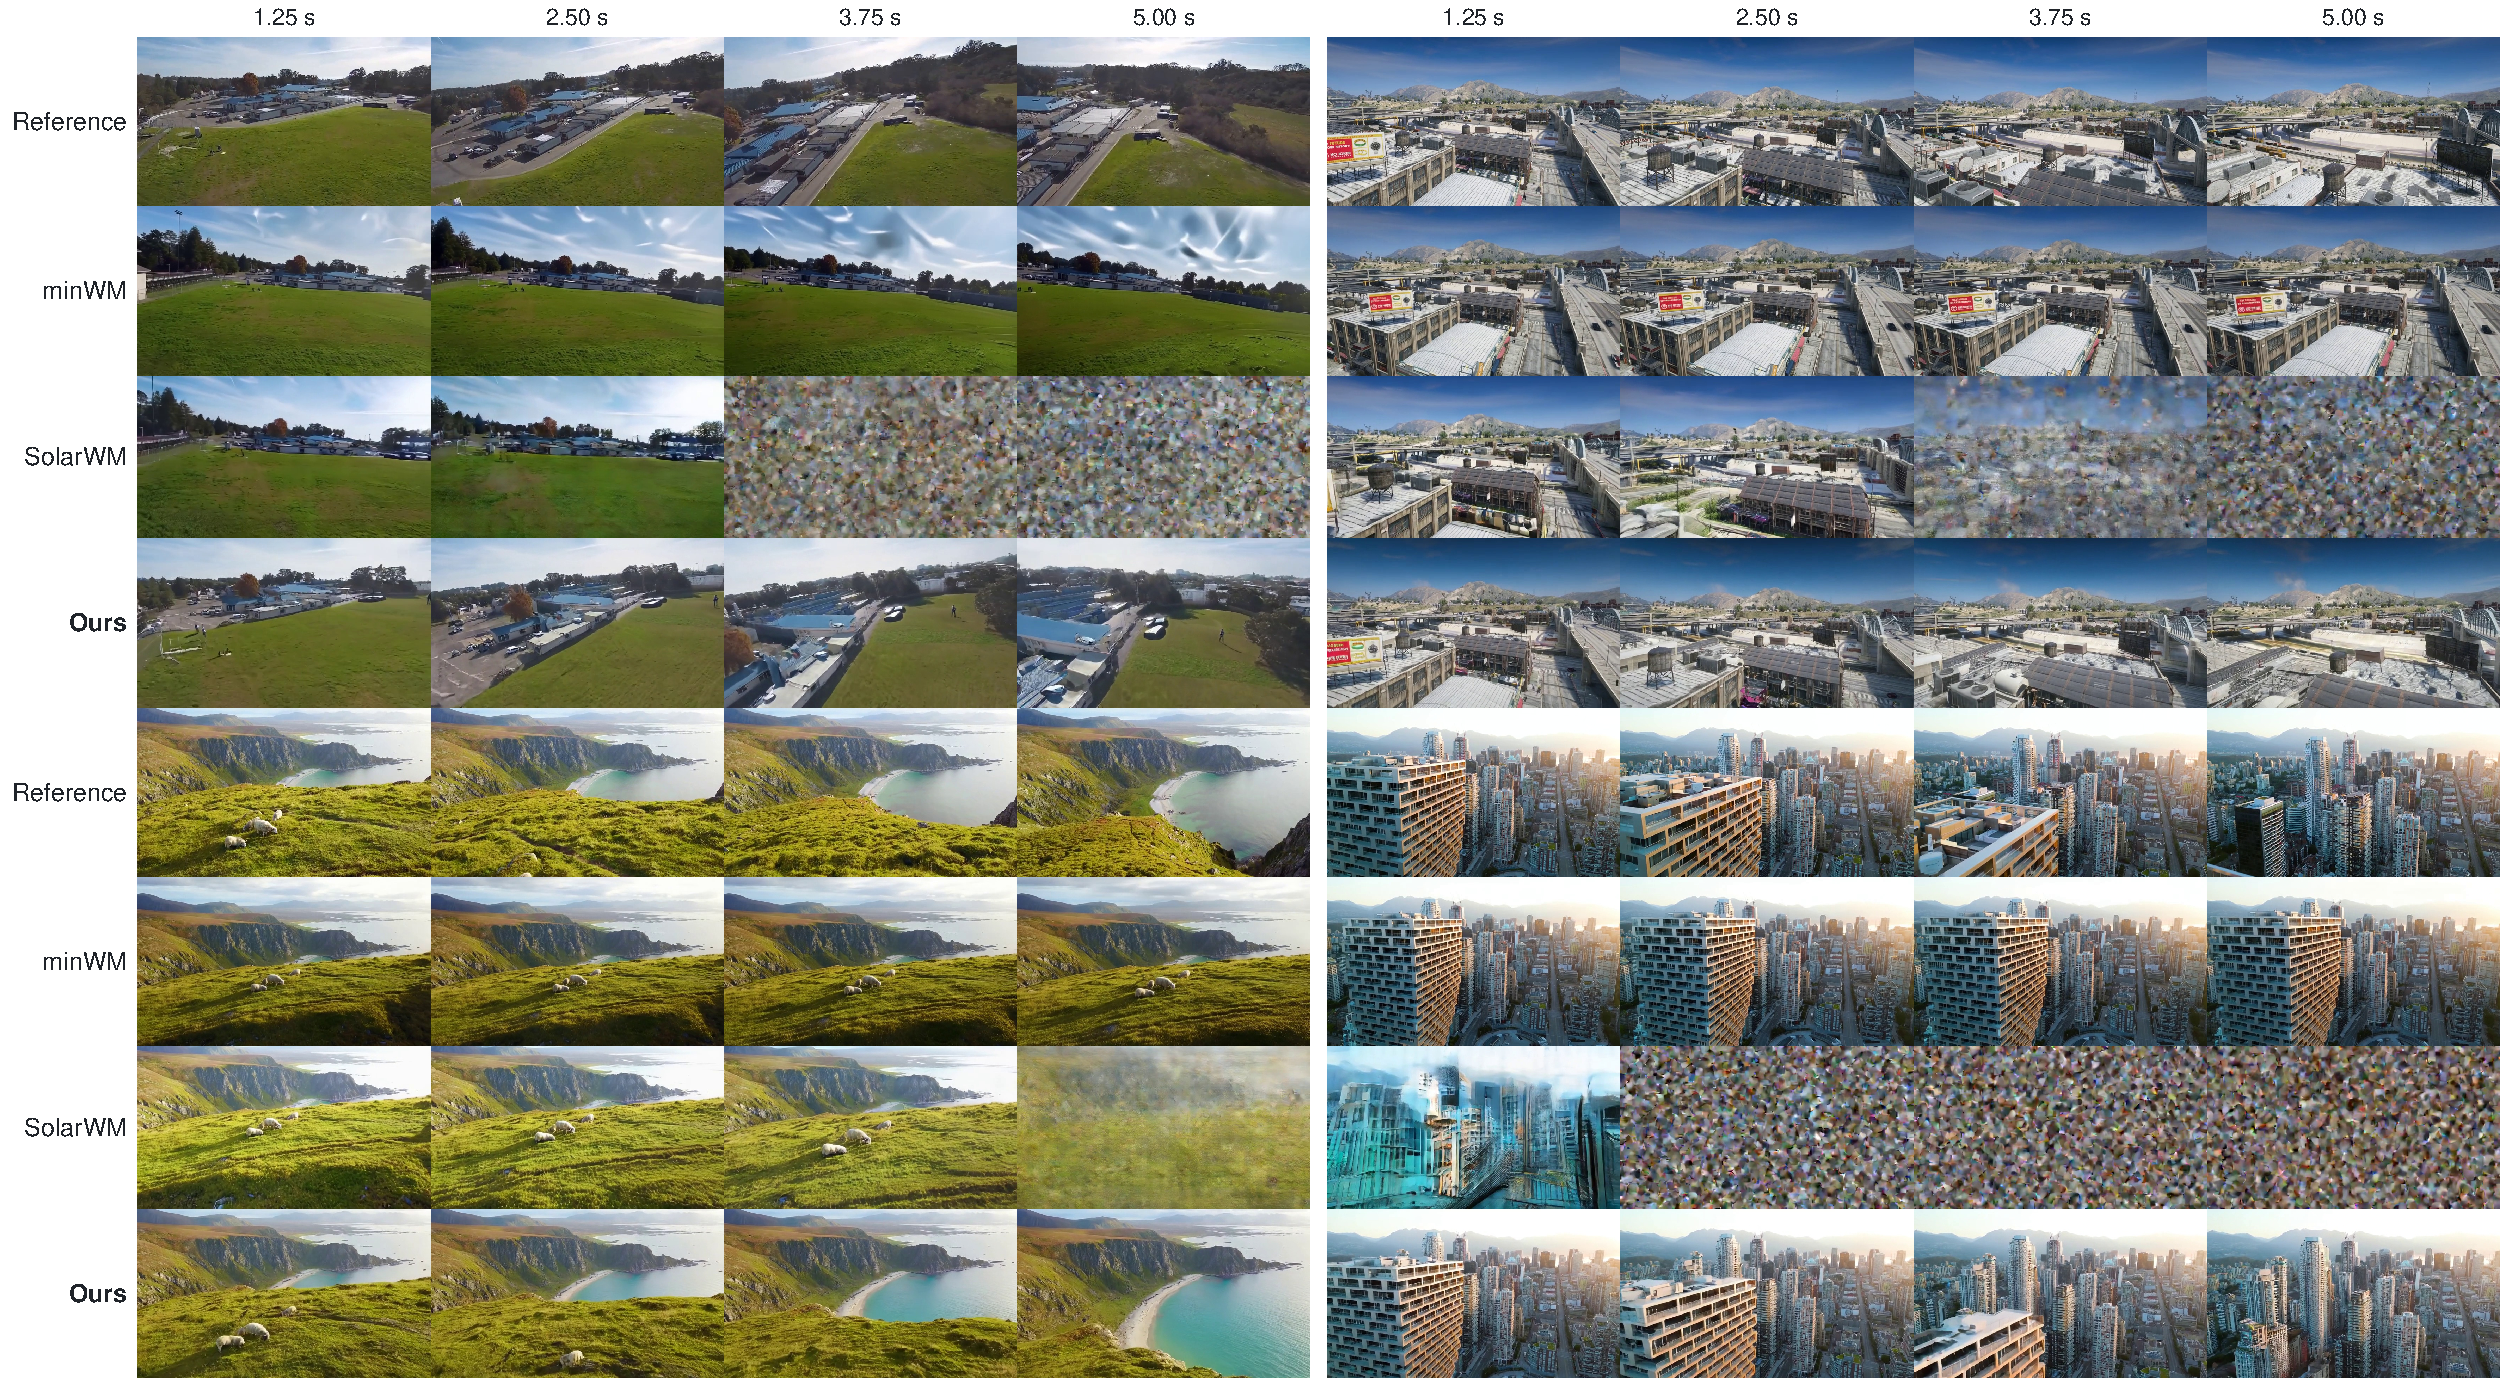
\includegraphics[width=\textwidth]{figures/qualitative_comparison.pdf}
    \caption{Qualitative comparison of camera-conditioned TI2V world models. The examples compare scene-structure preservation and viewpoint progression.}
    \label{fig:qualitative_comparison}
\end{figure*}

\paragraph{Depth accuracy and temporal consistency.}
We separately evaluate depth annotation on 16 GTA clips with reference depth, using all 81 frames per clip.
Table~\ref{tab:depth_annotation_selection} compares MetricAnything with the selected MetricAnything--VDA combination under RGB-only inference.
We average per-clip errors equally and measure temporal log-depth error along correspondences obtained from reference depth and camera motion.
VDA-guided stabilization reduces temporal error from 0.03759 to 0.02124, with AbsRel changing from 17.69\% to 18.20\% and RMSE from 9.54 to 9.63\,m.
The combination achieves the lowest temporal error among the evaluated configurations while maintaining similar per-frame depth accuracy.
The Supplementary Material includes the full focal-input comparison and evaluation protocol.

% Pose selection evidence: camera_trajectory_report.md, Sections 7.2, 7.3,
% 7.6, 7.7, and 7.9. Validation composition follows the author's correction
% to 12 GTA clips and four real-world clips. Common valid subsets are kept.
% Depth evidence: metric-depth-rgb-v1.0/evidence/nok_results.csv,
% protocol.json, and nok_protocol.json. This is a separate 16-GTA-clip panel.

\subsection{Quantitative comparison}
\label{sec:experiment_results}

Table~\ref{tab:main_comparison} shows that our model achieves the best scores across all reported metrics among the three evaluated checkpoints.
Compared with SolarWM, LPIPS decreases by 23.8\% and FVD by 69.7\%.

The visual gains are accompanied by more accurate camera control.
Relative to SolarWM, our model reduces rotation error by 62.9\% and normalized translation error by 32.6\%, while AUC@30 increases from 0.708 to 0.813.
Thus, on this evaluation panel, improved appearance is accompanied by closer adherence to the requested trajectory.
These comparisons evaluate complete systems; we examine the contribution of joint depth prediction separately in Sec.~\ref{sec:depth_ablation}.

\subsection{Depth ablation}
\label{sec:depth_ablation}

\begin{table}[t]
    \centering
    \caption{Depth ablation comparing RGB-only and joint RGB--depth generation. Appearance and camera-control metrics assess the contribution of depth supervision. Best results are bold.}
    \label{tab:depth_ablation}
    \small
    \setlength{\tabcolsep}{8pt}
    \begin{tabular}{@{}lrr@{}}
        \toprule
        Metric & RGB-only & RGB+Depth \\
        \midrule
        PSNR (dB)$\uparrow$ & 13.954 & \textbf{15.515} \\
        SSIM$\uparrow$ & 0.39115 & \textbf{0.43722} \\
        LPIPS$\downarrow$ & 0.40428 & \textbf{0.36595} \\
        FVD$\downarrow$ & 52.350 & \textbf{47.874} \\
        \midrule
        RotErr ($^\circ$)$\downarrow$ & 2.305 & \textbf{1.876} \\
        TransErr$\downarrow$ & 0.09501 & \textbf{0.08600} \\
        CamMC$\downarrow$ & 0.12069 & \textbf{0.10632} \\
        CosSim$\uparrow$ & 0.89129 & \textbf{0.99155} \\
        AUC@15$\uparrow$ & 62.26\% & \textbf{70.49\%} \\
        AUC@30$\uparrow$ & 72.98\% & \textbf{81.76\%} \\
        \bottomrule
    \end{tabular}
\end{table}

Table~\ref{tab:depth_ablation} compares RGB-only generation with joint RGB--depth generation to assess the contribution of depth prediction and supervision.
For this ablation, we additionally report PSNR and SSIM as complementary appearance metrics.
Joint generation improves both visual fidelity and camera control: LPIPS decreases by 9.5\%, rotation error by 18.6\%, and AUC@30 increases by 8.78 percentage points.
These results support joint depth prediction as useful geometric supervision for camera-conditioned video generation.

\subsection{Qualitative comparison}
\label{sec:qualitative_comparison}

% Selected scenes: 019, 021, 044, 066, 079, 093 in the author's review gallery.
% The Ours visualizations use step005427 live weights; the quantitative table
% retains the measured DF step252 results. The figure PDF is used unchanged.

Figure~\ref{fig:qualitative_comparison} shows six selected examples from real and simulated scenes.
In these examples, minWM often shows limited viewpoint change, while SolarWM sometimes loses scene structure in later frames.
Our outputs retain recognizable scene layouts across the displayed times while producing clearer viewpoint changes.
